\chapter{Introduction}
\label{cha:introduction}

This chapter aims to introduce the reader to the motivation that led to the project and the basic concepts to understand the rest of the sections. In addition, the objectives of this are defined, and, finally, the structure of the memory is detailed.

\section{Motivation}
\label{sec:motivation}

In 1996, data accumulated and rate at which new data was collected was already very fast. It was necessary to search for new techniques and tools to obtain useful information from all this data \cite{Fayyad96b}. Nowadays this data explosion continues to grow. It is even easier to collect and store data with current technology.

This causes larger and larger datasets to appear more often and a problem to know what are important and useful information. A high-dimensional dataset is a dataset that has a larger number of attributes or features ($p$) than the number of observations or instances ($N$). It can be expressed $p >> N$ \cite{high-dimensionality}.

High dimensionality entails a problem: it is very difficult to find a relationship between the predictor variables and the output variables. This is because there are not enough observations to train the model\footnote{Relationship models describe the types of connections/associations between buyers and suppliers, along with the interactions which occur over time as part of these relationships \cite{carr1999strategically}.} with which the relationship is obtained and a deterministic answer\footnote{The determinist answer is that features values has a cause and is thus predictable.} will not be found.

Different fields use high dimensional datasets. Some examples \cite{Dua:2019} are the following:
\begin{itemize}
    \item \textbf{Life Sciences:} \href{http://archive.ics.uci.edu/ml/datasets/gene+expression+cancer+RNA-Seq}{\textit{gene expression cancer RNA-Seq Data Set}} with 20531 attributes and 801 instances.
    \item \textbf{Physical Sciences:} \href{http://archive.ics.uci.edu/ml/datasets/Amazon+Commerce+reviews+set}{\textit{Amazon Commerce reviews set Data Set}} with 10000 attributes and 1500 instances.
    \item \textbf{\acrshort{cs} / Engineering:} \href{http://archive.ics.uci.edu/ml/datasets/YouTube+Multiview+Video+Games+Dataset}{\textit{YouTube Multiview Video Games Dataset Data Set}} with 1000000 attributes and 120000 instances.
    \item \textbf{Social Sciences:} \href{http://archive.ics.uci.edu/ml/datasets/A+study+of++Asian+Religious+and+Biblical+Texts}{\textit{A study of Asian Religious and Biblical Texts Data Set}} with 8265 attributes and 590 instances.
    \item \textbf{Business:} \href{http://archive.ics.uci.edu/ml/datasets/Farm+Ads}{\textit{Farm Ads Data Set}} with 54877 attributes and 4143 instances.
    \item \textbf{Other:} \href{http://archive.ics.uci.edu/ml/datasets/Trains}{\textit{Trains Data Set}} with 54877 attributes and 4143 instances.
\end{itemize}

A solution is \acrfull{dm}. \acrshort{dm} is the process of uncovering patterns and other valuable information from large datasets \cite{data-mining}. It is a step of \acrfull{kdd} process. The main objectives are (i) to automate the process of finding useful patterns in data and (ii) find comprehensible models. Data  mining techniques can describe the target dataset. Outcomes can be predicted through the use of \textbf{machine learning} algorithms.

\section{KDD Process}
\label{sec:kdd-process}

The \acrlong{kdd} process refers to the process of identifying valid, novel, potentially useful, and primarily understandable patterns in a dataset. It comprises several stages: preprocesing (including recopilation, selection, cleaning and transformation), \acrlong{dm}, model evaluation and deployment (including model interpretation, use, dissemination and monitoring) \cite{Hernandez-Orallo05a}.

In an attempt to normalize this knowledge discovery process, a main methodology emerged: \acrfull{crisp-dm}.

\acrshort{crisp-dm} is a proven method for targeting your \acrshort{dm} jobs. It includes descriptions of the normal phases of a project, the tasks required in each phase, and an explanation of the relationships between the tasks. Figure \ref{fig:crisp-dm} shows the stages of these methods. It has the following characteristics:
\begin{itemize}
    \item In this case, \acrlong{dm} is just one stage of the process. Sometimes it is used to name the entire process.
    \item The cycle consists of six phases: Problem Domain, Data Understanding, Preprocesing, \acrlong{dm}, Evaluation and Deployment.
    \item The arrows between phases represent the most common flow but it is usual to go back and forth in the phases as needed for the project.
    \item \acrshort{crisp-dm} allows you to create a \acrshort{dm} model that suits your specific needs because it is flexible and can be easily customized.
    \item It integrates all the necessary tasks in \acrshort{dm} projects, from the phase of understanding the problem to the start-up of automated analytical, predictive and/or prospective systems.
    \item The outer circle in the Figure \ref{fig:crisp-dm} symbolizes the cyclical nature of data analysis projects. The information discovered during the process and the deployed solution can produce new iterations of the model.
\end{itemize}

\begin{figure}[H]
    \centering
    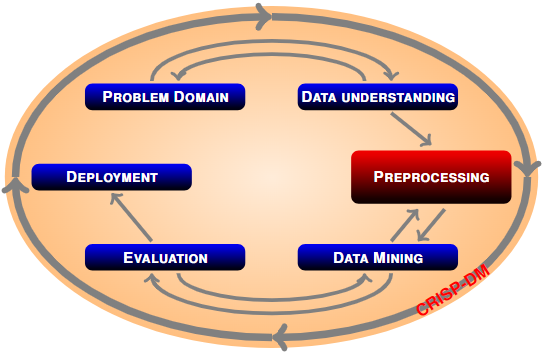
\includegraphics[scale=2]{crisp-dm.png}
    \caption{\acrshort{crisp-dm}.}
    \label{fig:crisp-dm}
\end{figure}

The first stage is \textbf{Problem Domain}. Every \acrshort{dm} project should start with a profundity understanding of the problem to be solved and establish the requirements and objectives of the project from a business perspective and then translate them into technical objectives and a project plan.

The stage number two is \textbf{Data Understanding}. The collection and initial exploration of the data is carried out with the aim of establishing a first contact with the problem. This stage is usually critical in the project since a misunderstanding of the data results in an increase in the overall time of the project and also reduces the guarantees of success.

The next and third stage is \textbf{Preprocessing}. This stage is about selecting, cleaning and generating correct datasets, organized and prepared for the \acrshort{dm} phase. It is extremely critical in a \acrshort{dm} project. Errors in the data that are overlooked and not resolved in this phase are carried over to the \acrshort{dm} stage, leading to a reduction in the accuracy of the models or even the possibility of delivering results based on data to the client. data that still contains undetected errors. For this reason, this phase is crucial and generally always demands the greatest effort and time of the project. This stage is highlighted in red in the diagram of Figure \ref{fig:crisp-dm} because it will be the part that we will work on later in this project.

\textbf{\acrlong{dm}} is the fourth stage. Knowledge models are created from the data supplied from the previous stage. These knowledge models can be of different types, for example, classification or regression models can be created with the aim of estimating or inferring the value of a certain variable. To face this phase, a series of guidelines must be followed. First, the most appropriate modeling algorithms for the problem are selected and then a test plan is generated, where the values of the parameters that will be used for the machine learning algorithms are configured. Finally, the models are built, executing the selected algorithms on the prepared data.

The fifth stage is \textbf{Evaluation}. It is checked whether the models obtained in the previous stage meet the objectives and business expectations set out in the problem domain stage. If it is not satisfactory, it proceeds to iterate again over the previous steps in order to find new results.

The last stage is \textbf{Deployment}. It is where the strategies for its implementation, monitoring and maintenance of the models are defined. This will help to observe any irregular behavior of the system and correct it in a way that does not cause deficiencies in customer service. To conclude, a final review of the entire process is carried out, evaluating the actions carried out correctly and incorrectly, in order to list the lessons learned in the project.

As a conclusion-summary, Table \ref{tab:crisp-dm} presents a guide to all the stages and the tasks that are carried out in each of them.

\begin{table}[H]
    \begin{center}
        \begin{tabular}{| c | c |}
            \hline
            \textbf{Stages} & \textbf{Tasks} \\ \hline
            \multirow{6}{*}{\textbf{Problem Domain}} & \\ 
             & Determinate Business Objectives \\
             & Assess Situation \\
             & Determine Data Mining Goals \\
             & Produce Project Plan \\
             & \\ \hline
            \multirow{6}{*}{\textbf{Data Understanding}} & \\
             & Collect Initial Data \\
             & Describe Data \\
             & Explore Data \\
             & Verify Data Quality \\
             & \\ \hline
            \multirow{6}{*}{\textbf{Preprocessing}} & \\
             & Recopilate Data \\
             & Clean Data \\
             & Tranformate Data \\
             & Reduce Data \\
             & \\ \hline
            \multirow{6}{*}{\textbf{Data Mining}} & \\
             & Select Modeling Technique \\
             & Generate Test Design \\
             & Build Model Parameter Settings \\
             & Assess Model \\
             & \\ \hline
            \multirow{5}{*}{\textbf{Evaluation}} & \\
             & Evaluate Results \\
             & Approved Models \\
             & Determine Next Steps \\
             & \\ \hline
            \multirow{6}{*}{\textbf{Deployment}} & \\
             & Plan Deployment \\
             & Plan Monitoring and Maintenance \\
             & Produce Final Report \\
             & Review Project \\ 
             & \\ \hline
        \end{tabular}
        \caption{Specific tasks of \acrshort{crisp-dm} stages \cite{visual-crisp-dm}.}
        \label{tab:crisp-dm}
    \end{center}
\end{table}

\subsection{Preprocessing}
\label{sec:preprocessing}

\textbf{Preprocessing} is the third stage of \acrshort{crisp-dm} method. It is also known as \textbf{Data Preparation}. It is one of the most important parts of \acrshort{kdd} process. Preprocessing is often the most time-consuming stage, estimated to usually takes 50-70\% of a project's time and effort \cite{preprocessing-time}. It covers all the activities to build the dataset to be used for further processing from the initial data. These activities or tasks can be performed several times and in no particular order.

Data Preparation ensures that the dataset used for the modeling stage is acceptable and of better quality. Data comes from a multitude of sources, can be high dimensionality, and have a wide variety of attributes. Real-world data is generally noisy, incomplete, and inconsistent. It means that the raw data tends to be corrupted, has missing values or attributes, outliers, or conflicting values. Therefore, preprocessing prevents analytical models from receiving poor quality data that can lead to misleading predictions.

Figure \ref{fig:preprocessing} shows a scheme of the main activities involved in Data Preparation. They are Data Recopilation, Data Cleaning, Data Transformation and Data Reduction.

\begin{figure}[H]
    \centering
    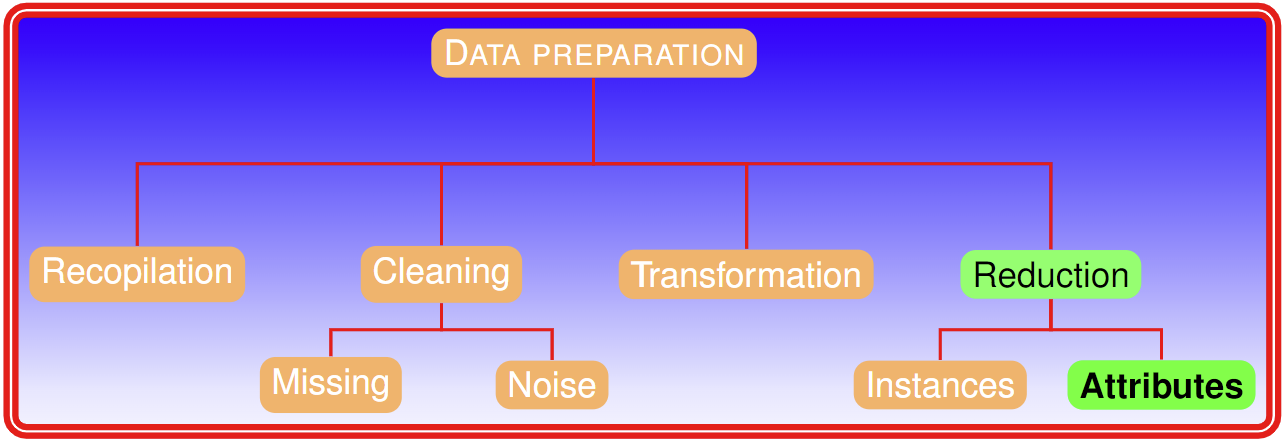
\includegraphics[scale=1.3]{preprocessing.png}
    \caption{Main activities of Data Preparation.}
    \label{fig:preprocessing}
\end{figure}

\textbf{Recopilation} task focuses in joining data about the same object but that are scattered in different sources, combining multiple tables or records to create new ones. Aggregations can be made, which summarize the information contained in several of those records.

\textbf{Cleaning} task includes inserting suitable default values to estimate missing values or ignore respective records having \textbf{missing values or features}. This task also cover deletion of duplicate or redundant records. To eliminate \textbf{noise} is usual apply regression to smooth or curve fit or apply clustering to identify and eliminate it.

\textbf{Transformation} task consists of generating derived attributes, new records or transformed values of existing attributes from the originally captured data based on the requirements to prepare the input to the modeling tools. There may be attribute order requirements, or the modeling tool may require records to be ordered by the resulting attribute.

\textbf{Reduction} task makes easy to handle and produce similar analytical results when reducing data. There are two types of reduction. We can reduce number of instances to have smaller data representations or dimensionality to eliminate insignificant attributes. \textbf{Instances reduction} is achieved with methods such as record sampling, clustering or regression. On the other hand, \textbf{attributes reduction} is carried out with processes such as attribute sampling, the heuristic method or, the most important for this project, \textbf{feature selection}.

\section{Feature Selection}
\label{sec:feature-selection}

\acrfull{fs} is the process of reducing the number of input variables when developing a predictive model. It is desirable to reduce the number of input variables to both reduce the computational cost of modeling and, in some cases, to improve the performance of the model \cite{fs-method-ml}.

As a result, reducing the number of variables yields the following benefits:
\begin{enumerate}
    \item With less data, data mining algorithms learn faster.
    \item Less misleading data means better modeling accuracy.
    \item \acrshort{fs} makes for better performance, which leads to better generalization.
    \item Simpler models makes it easier to understand.
    \item If there are less attributes, there is no need to collect such data.
    \item Reducing the measurement and storage requirements.
\end{enumerate}

\acrshort{fs} consists of choosing from the input variables those that are most relevant. Variables sometimes are ordered in the form of a matrix where the columns are the variables and the rows are the instances. This matrix is known as feature matrix.

There are different algorithms that are responsible for selecting the features that seem relevant to them. Not everyone takes the same features as important. Different algorithms can select different variables, that is, different columns of the feature matrix. Depending on the algorithm used, the selected features change.

\section{Objectives}
\label{sec:objectives}

You can measure how stable different \acrshort{fs} algorithms are on a given dataset. For that reason, there are different data complexity metrics and \acrshort{fs} stability metrics.

Study of data complexity metrics is an emergent area in the field of data mining and is focused on the analysis of several data set characteristics to extract knowledge from them \cite{CANO20134820}.

Stability is defined as the sensitivity of a method to variations in the training set \cite{Kalousis2007}. An algorithm is `unstable' if a small change in data leads to large changes in the chosen feature subset \cite{JMLR2018}.

The fundamental objective of this project is the study and analysis of different feature selection algorithms in real datasets.

The specific objectives of this project are the following:

\begin{itemize}
    \item Carry out a study of "classical" \acrshort{fs} algorithms.
    \item Know available defect prediction datasets.
    \item Apply \acrshort{fs} algorithms to datasets.
    \item Measure stability.
    \item Measure complexity.
    \item Know about SHAP values.
\end{itemize}

\section{Structure}
\label{sec:structure}

This document has different chapters in which the most relevant information about the development carried out in this project is collected, as well as the theoretical foundations required for the understanding of this memory. Each of these chapters is briefly described below:
\begin{itemize}
    \item \textbf{Chapter 1: Introduction.} This chapter begins with the motivation of the project, the explanation of some of the most important concepts, the objectives that are carried out and this section where the structure of the rest of the project is detailed.
    
    \item \textbf{Chapter 2: Theoretical Study.} This chapter aims to give a detailed overview of the most important ideas of the topic that this project deals with. It will delve into the types of \acrshort{fs} and other concepts such as complexity or stability.
    
    \item \textbf{Chapter 3: Experimental Work.} In this chapter, various \acrshort{fs} R packages are chosen and tested on defect prediction datasets. The complexity and stability of some of the results obtained are also measured.
    
    \item \textbf{Chapter 4: Conclusions and Future Work.} This chapter summarizes what has been learned, gives an opinion on what has been developed and personal conclusions are obtained from the work carried out. Finally, some ideas are named that can be carried out in a future extension of this project.
    
    \item \textbf{Bibliography.} Set of references that have been made during the document.
    
    \item \textbf{Appendix A. Tools and resources.} The different tools used are named.
    
    \item \textbf{Appendix B. R and RStudio installation.} Explain how to install R and RStudio.
    
    \item \textbf{Appendix C. How to install and load packages in R.} Explanation of different ways to install and load required packages.
    
    \item \textbf{Appendix D. Tables of Feature Selection in FSinR.} Results of \acrlong{fs} in tables.
\end{itemize}